\chapter{Motivation} \label{cha:motivation}
Communicating knowledge and intentions through persistent visual means is maybe one of the most distinct features that separates humans from other animals.  Our ability to intuitively understand abstract representations created by other humans from distant places or times has shaped the world's history in unimaginable ways.  The fundamental reason for creating these representations, converying information to other humans, has not changed between the earliest cave paintings 40000 years ago (see \fref{fig:motivation:vis:cave}) and modern visualizations (see \fref{fig:motivation:vis:modern}).  While the direction of causality is unclear, the connection between humanity's focus on using visual represerntations to share knowledge and being exceptionally good at intepreting visual language by dedicating a large portion of our brain to this task is certaintly connected.  It is partially because of this reason why our global culture has spent so much effort and time on perfecting visual languages and metaphors.  However, an image can never contain the full information and, as such, a good visualization is like a story;  the designer provides all the necessary components, but the final assembly occurs in mind of the beholder and is, thus. ultimately subjective.

Good visualizations make subconcious use of some of the remarkable aspects of human perception.  We are capable of analyzing scenes both preattentively as well as attentively.  Preattentive perception happens when features of an image \emph{pop out}, or are obvious to the observer without conscious effort and is largely independent of the number of objects that are involved.  \fref{fig:motivation:gestalt} shows an example of this effect using the Gestalt theory~\cite{wertheimer1922untersuchungen}.  In his work, Wertheimer found that attributes such as closure, similarity, or continuation enable an observer to perceive a collection of objects as a continuous form (or \emph{Gestalt}).  He also investivated what objects can be added to these groupings before the continuous form is destroyed.  Understanding these fundamental truths about human perception are invaluable in creating meaning full visualizations;  40000 years ago or today.

\begin{figure}
  \centering
  \begin{subfigure}{\abtwoimagewidth}
    \fbox{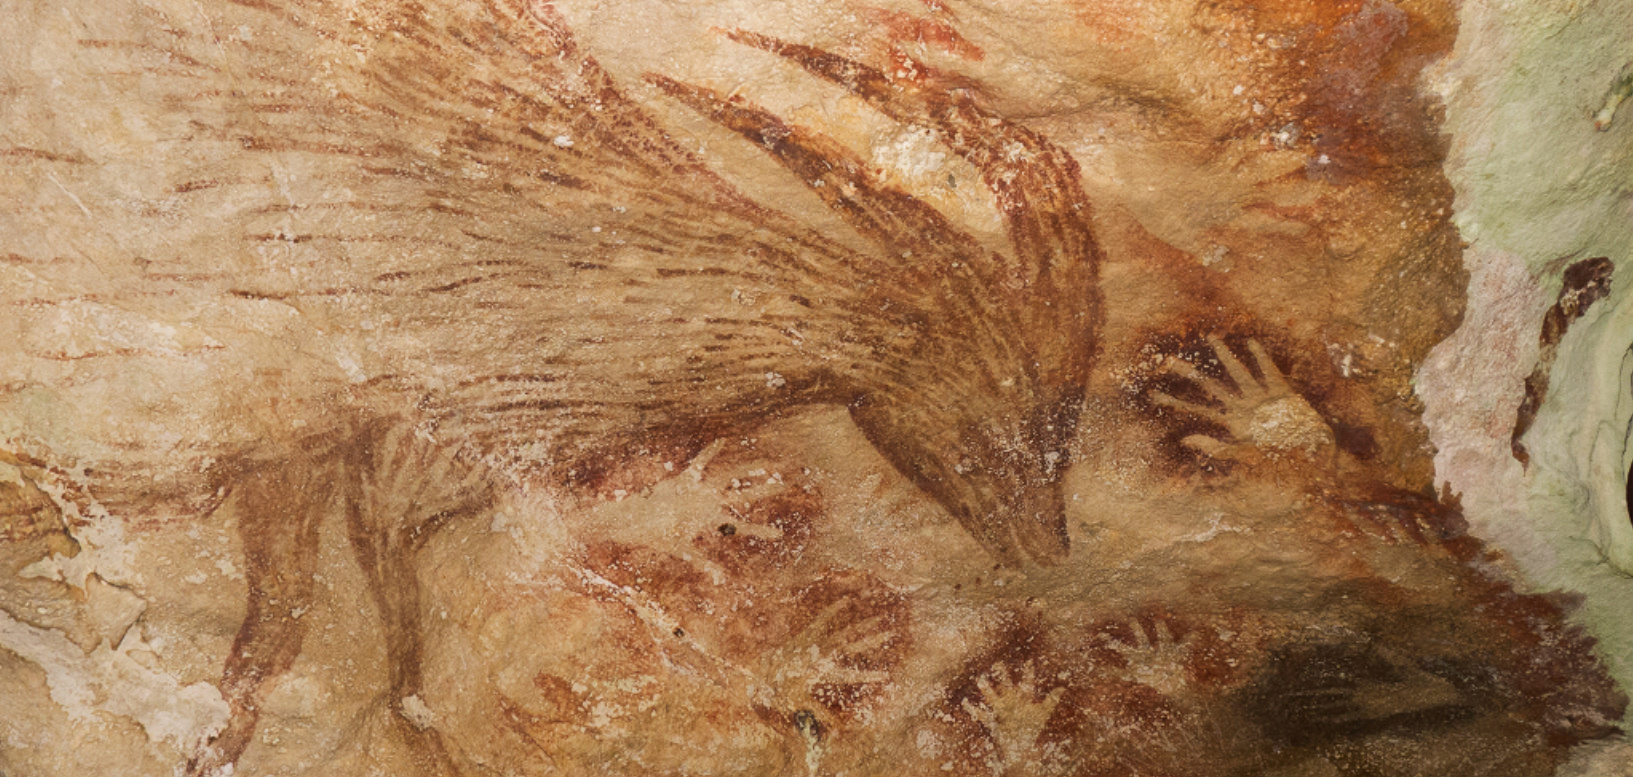
\includegraphics[width=\abfboximagewidth]{figures/motivation/cave.jpg}}
    \caption{The earliest known human cave painting from around 38000 BCE. Image copyright by Maxime Aubert.}
    \label{fig:motivation:vis:cave}
  \end{subfigure}
  ~
  \begin{subfigure}{\abtwoimagewidth}
    \fbox{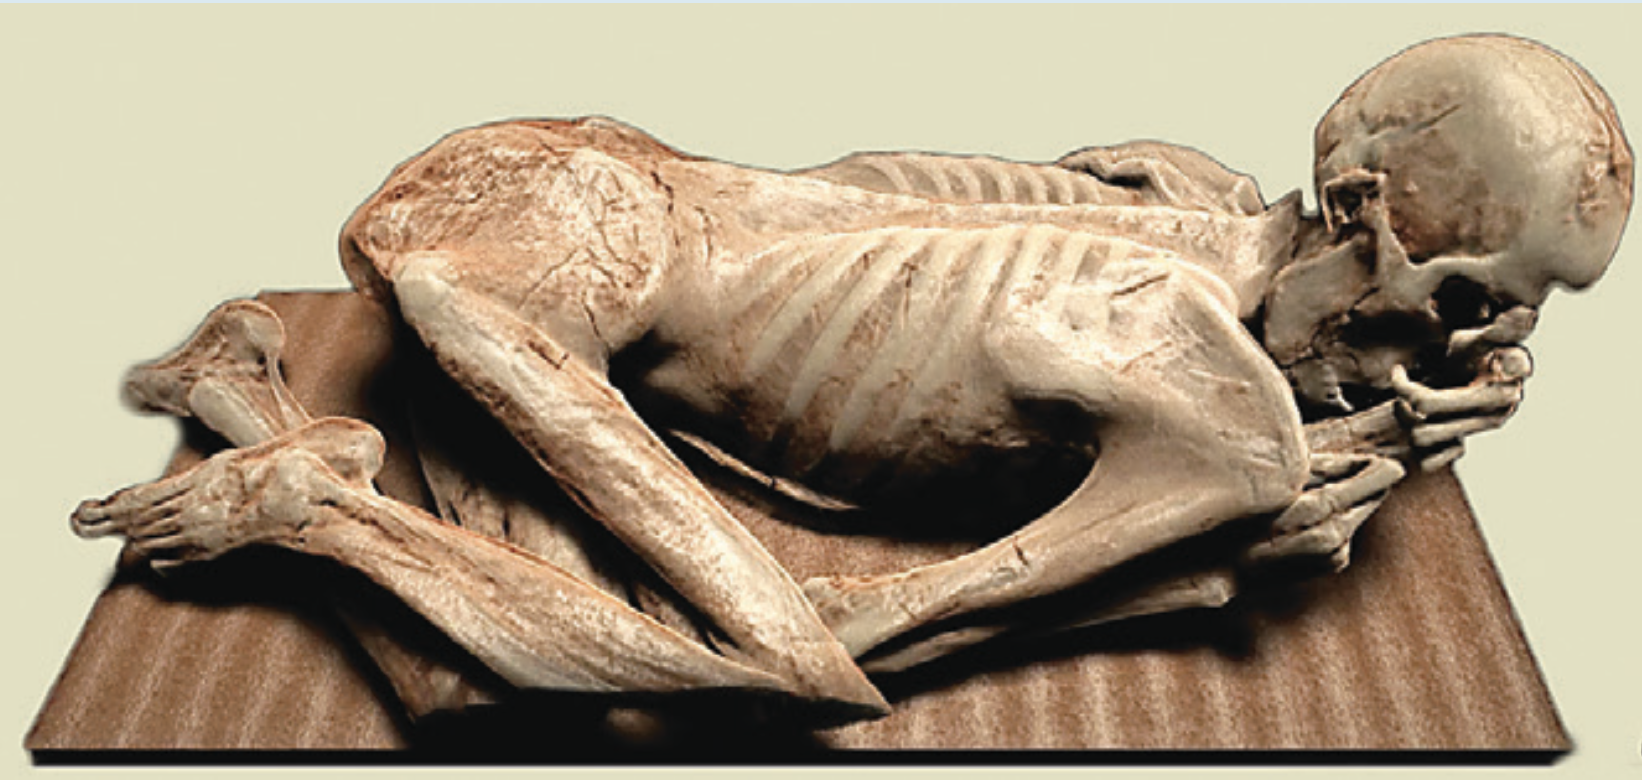
\includegraphics[width=\abfboximagewidth]{figures/motivation/gebelein.png}}
    \caption{A visualization using modern techniques of a pre-dynastic Egyptian mummy. Image copyright by Daniel J\"onsson.}
    \label{fig:motivation:vis:modern}
  \end{subfigure}
  \caption{Two examples of visualizations created by humanity that are 40000 years apart.  While the technological methods changed drastically, the ultimate purpose of conveying information to other humans remains the same.}
  \label{fig:motivation:vis}
\end{figure}

\begin{figure}
  \centering
  \begin{subfigure}{\abtwoimagewidth}
    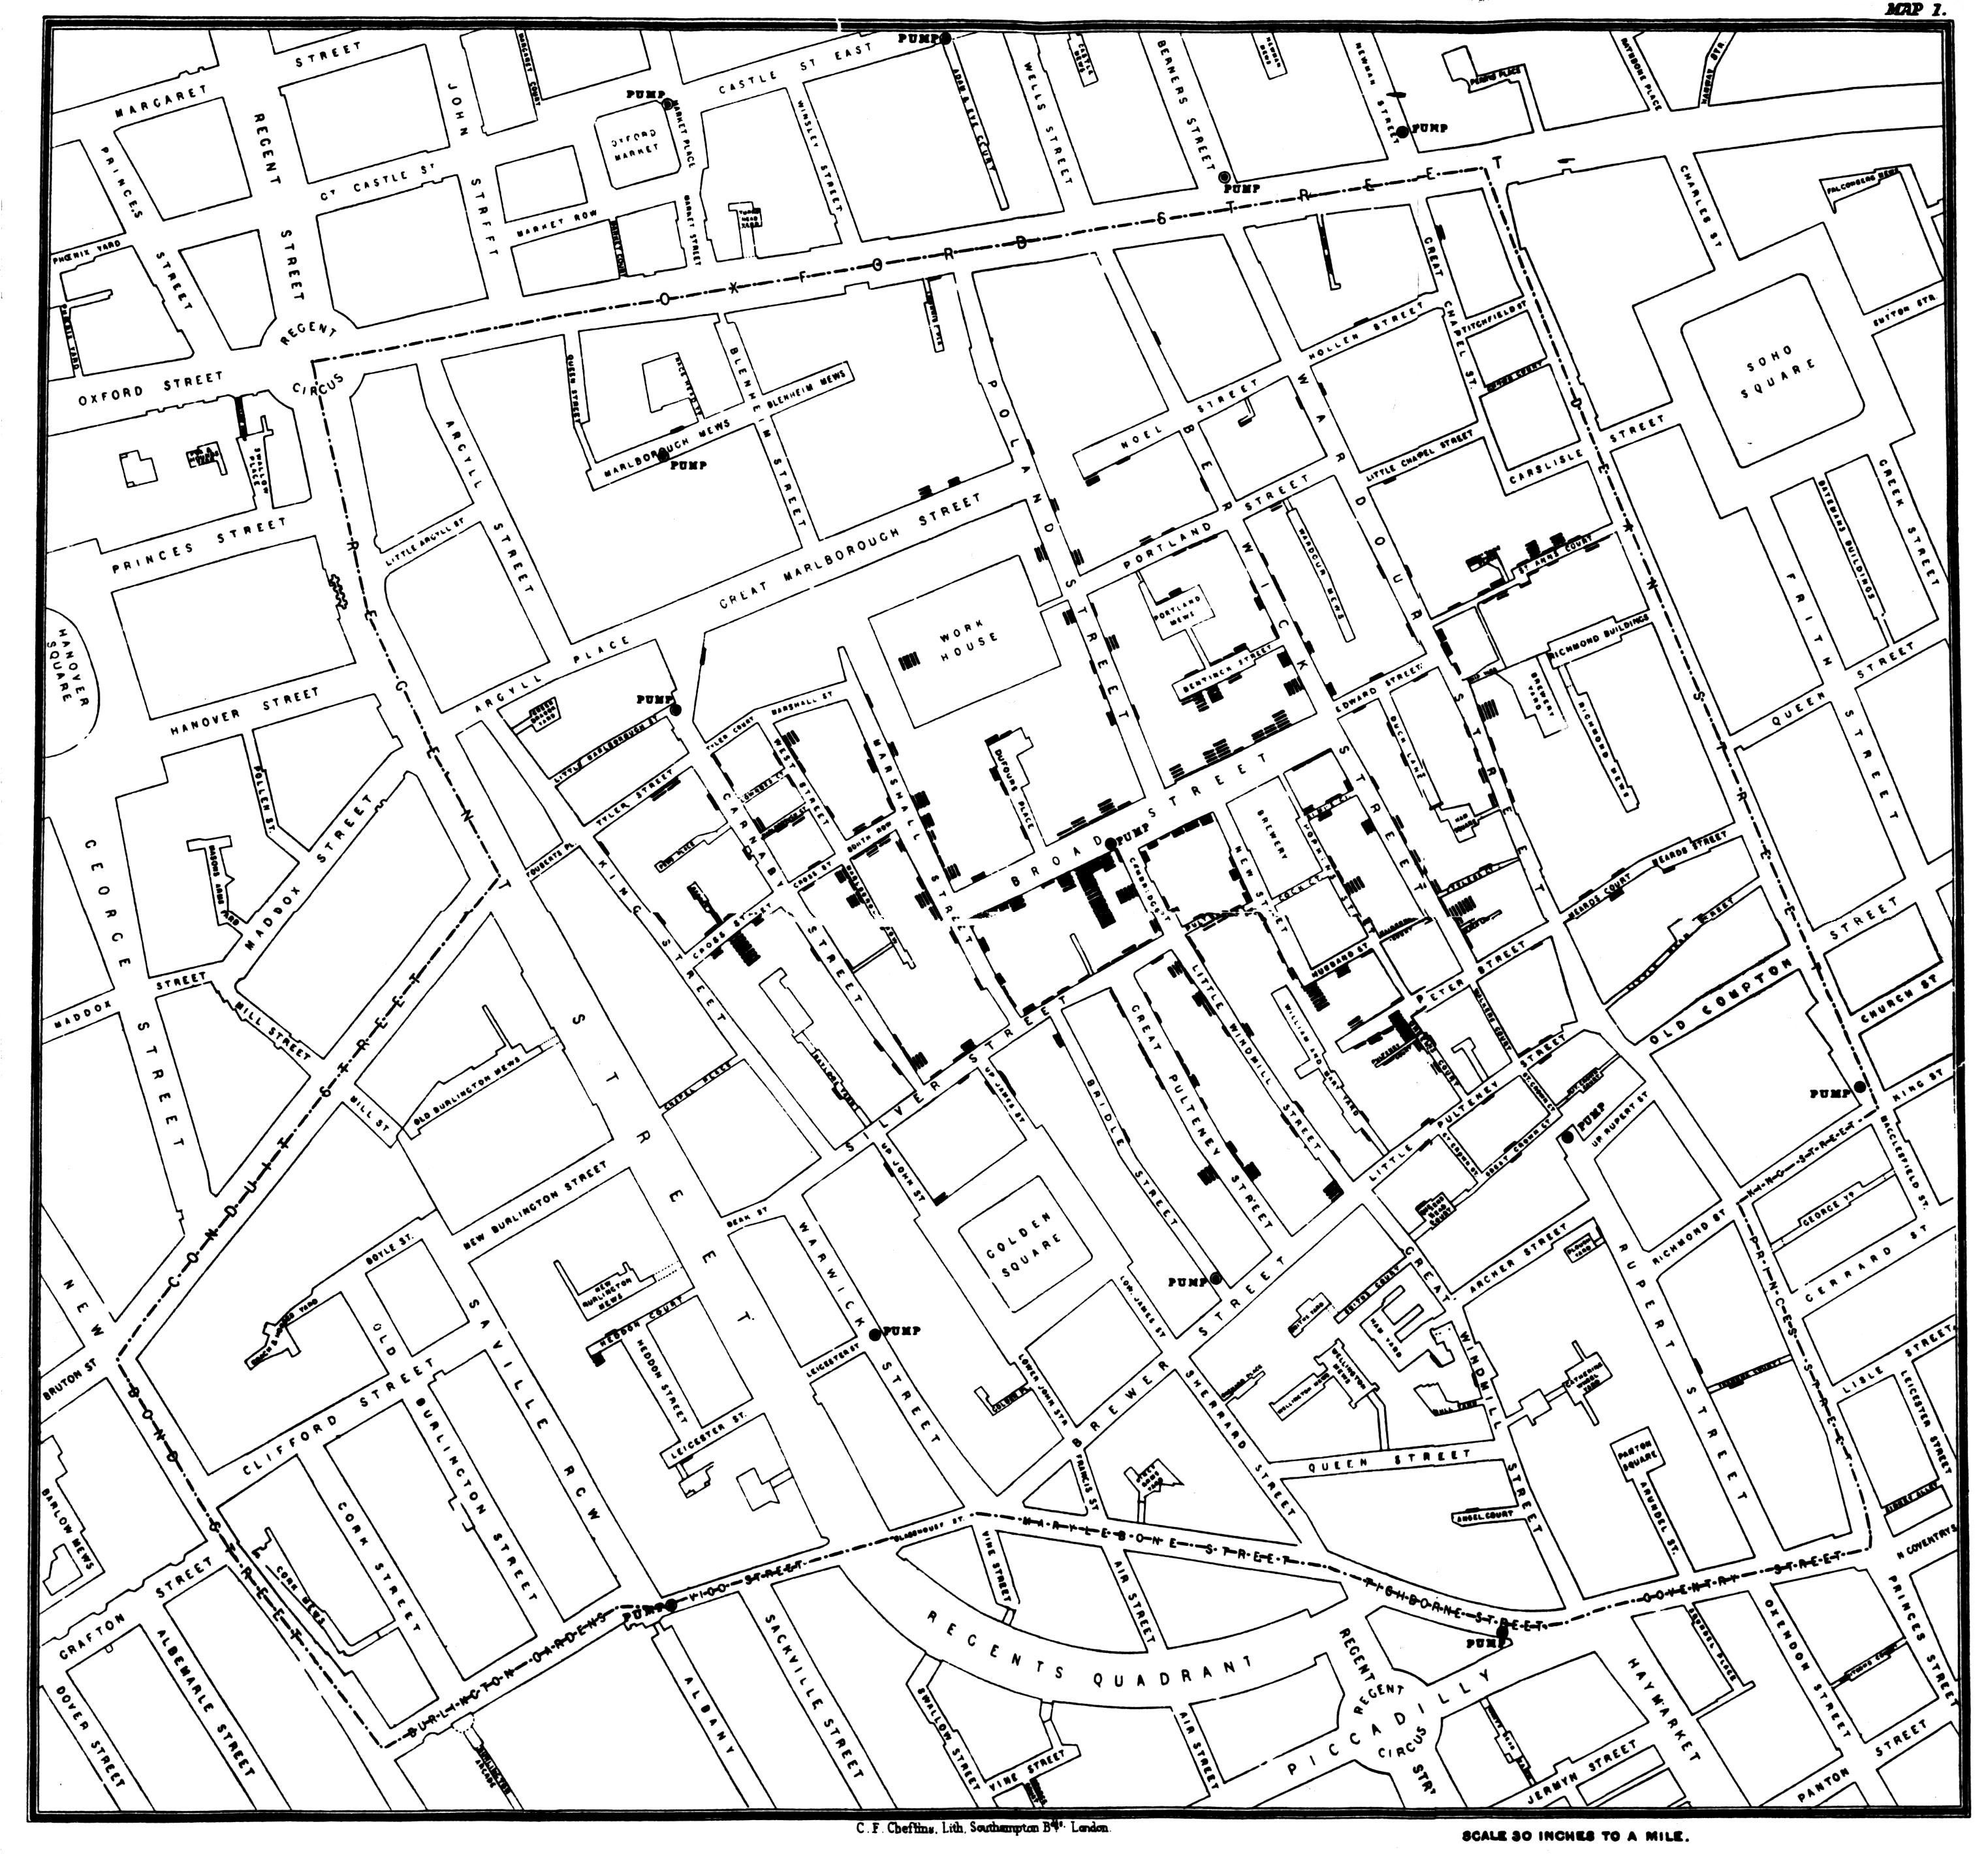
\includegraphics[width=\abfboximagewidth]{figures/motivation/cholera.jpg}
    \caption{A visualization of the spatial distribution of cholera outbreaks around Broad Street in London in 1854.}
    \label{fig:motivation:example:cholera}
  \end{subfigure}
  ~
  \begin{subfigure}{\abtwoimagewidth}
    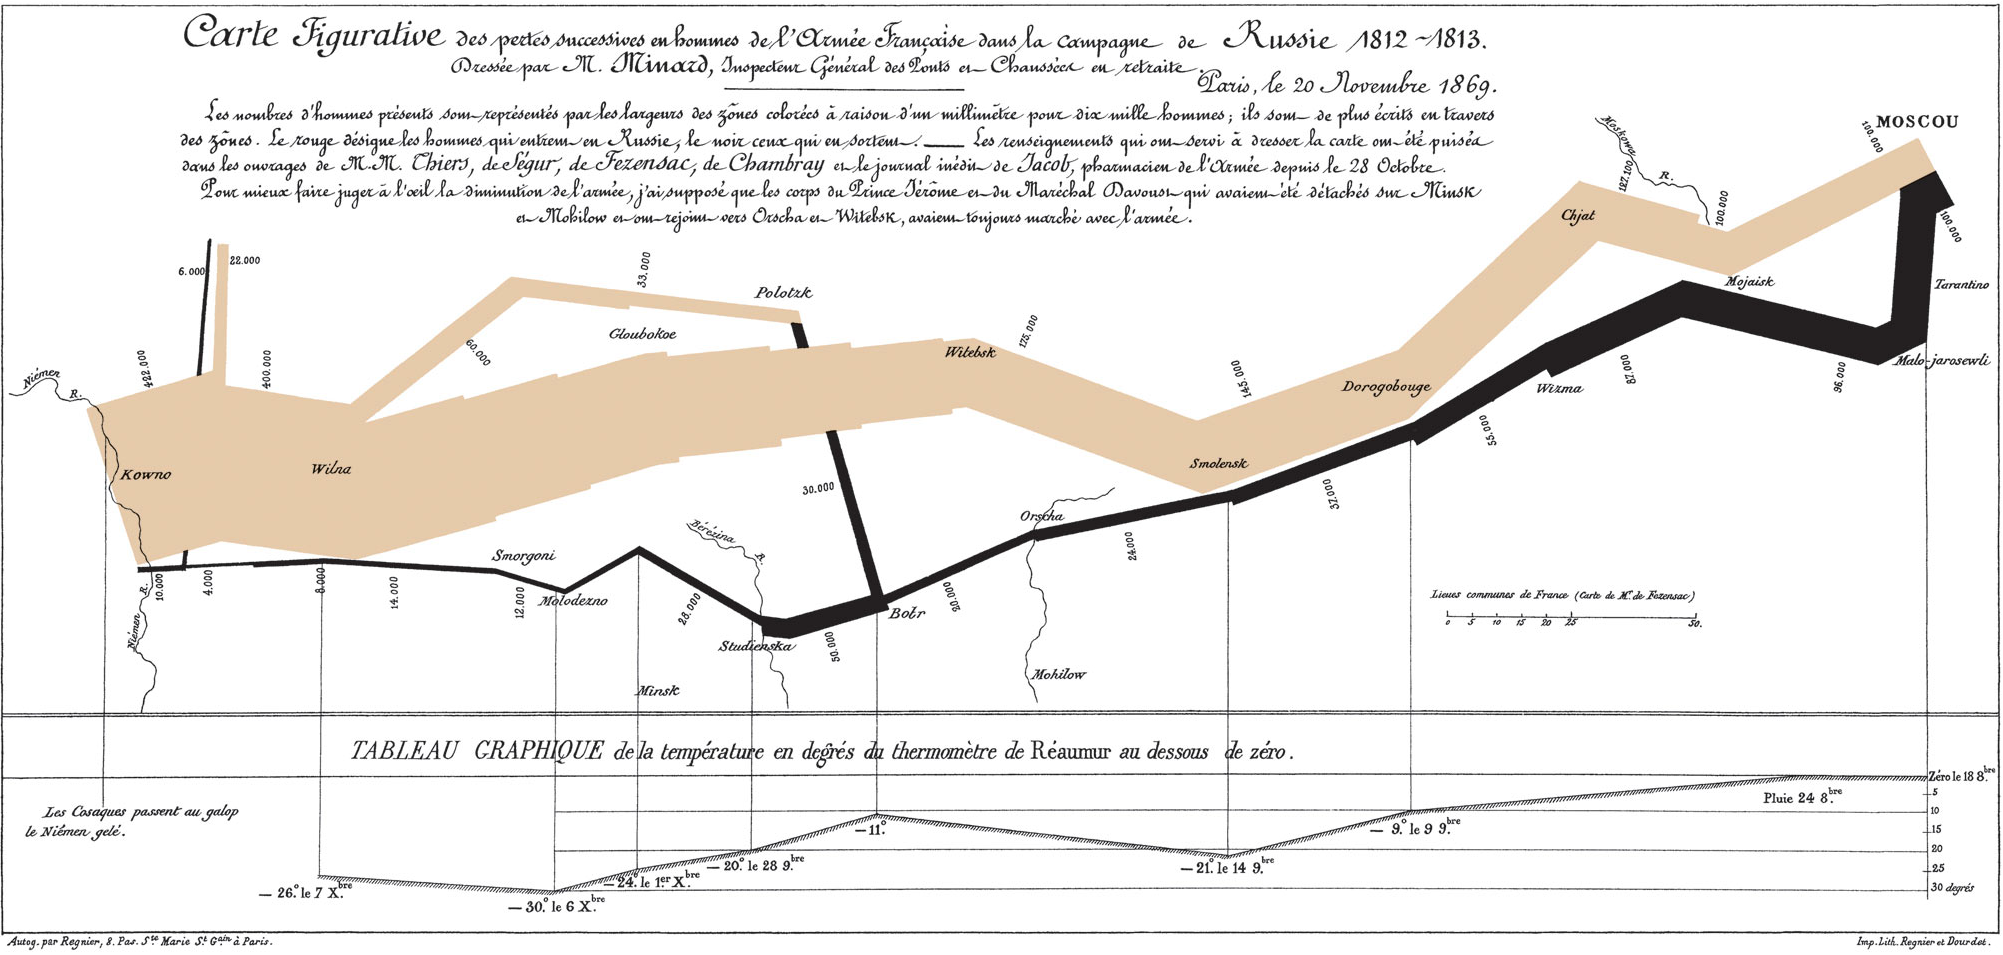
\includegraphics[width=\abfboximagewidth]{figures/motivation/napoleon.png}
    \caption{A multivariate visualization of Napoleon's campaign to Russian and reteat from Moscow in 1812-1813.}
    \label{fig:motivation:example:napoleon}
  \end{subfigure}
  \caption{Two well-known examples of visualization used to produce scientific insight (a) and provide public with a method to understand complex, multivariate data (b)}
  \label{fig:motivation:example}
\end{figure}

An early example of the successful use of visualization for the public good is a spatial map of the cholera outbreaks around Broad street in London in 1854 (see~\fref{fig:motivation:example:cholera}).  The prevelant theory at the time for transmission of diseases was miasmatic, caused by bad air, and not caused by germs.  Many decades before Wertheimer's publication of Gestalt theory, John Snow already made use of its concepts to gain insights about the spatial distribution of these cholera cases.  He marked all cholera cases on a map and used this visualization to pinpoint the origin of the outbreak --- an infected pump~\cite{snow1855mode}.  While this visualization seems simple by today's standards, it was an important step towards establishing the germ theory of diseases.  This is a clear example of a knowledge-driven approach, where a visualization is used to generate and test a hypothesis and make gain an understanding of the available data.

Only a few years later, another example was created by Charles Joseph Minard in 1861 to visualize Napoleon's Russia campaign and the following retreat from Moscow in 1812 (\fref{fig:motivation:example:napoleon}).  The map shows six different variables: geography, time, temperature, the movement of Napoleon’s army, and the remaining number of troops.  The layout, design, and its ability to easily show Napoleon's fate in Russia has caused this graphic to be called ``the best statistical graphic ever drawn''~\cite{tufte1983visual}.  As this data was produced from previously published work and mainly aimed at the general public, it serves as an example as to how visualization can be used to explain highly complex data to a public that possibly only has cursory knowledge about the topic.  Besides these two examples, Tufte, in his books, provides many more good examples of visualization mixing design and information reprensentation~\cite{tufte1991envisioning}.  All of these examples show an important difference in purpose between visualization and computer graphics, which is also exemplified in Ben Shneiderman's quote that ``the purpose of visualization is insight, not pictures''~\cite{card1999readings}.  Instead of generating beautiful images devoid of information, the purpose of visualization is to create images that enable some person to derive insight from data.  While the concept of \emph{insight} is easily understood colloquially, a formal definition of it has sofar been elusive~\cite{north2006toward}.

\begin{figure}
  \centering
  \fbox{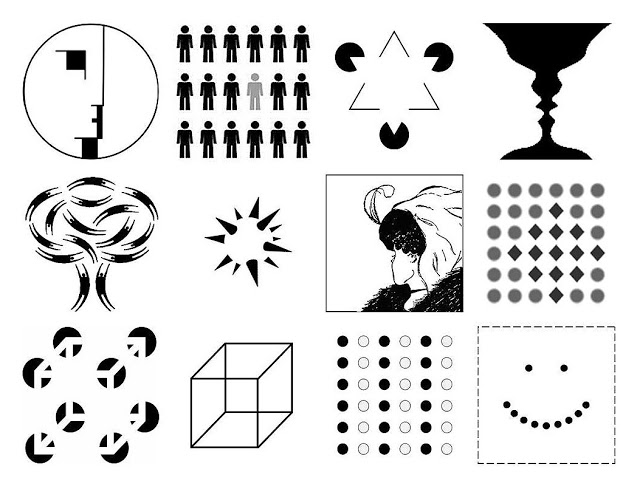
\includegraphics[width=\abfboximagewidth]{figures/motivation/gestalt.jpg}}
  \caption{Examples of Gestalt theory $\cdots$ Change image}
  \label{fig:motivation:gestalt}
\end{figure}

As alluded to in the two examples provided above, visualization cannot realistically occur without considering a specific \emph{target domain} or \emph{problem domain}.  A large portion of visualization research has to take the problem domain into account and is meaningless without this context.  Even for fundamental research, its effectiveness with regards to humans is important and has to be shown.  The different domains are frequently addressed through visualization applications that are tailored to an individual \emph{domain expert} or a group experts, who are interested in understanding a particular aspect of their data.  These experts can make use of visualization for either hypothesis generation, validation, or the communication of their theories.

Thus, the field of visualization is inherently an multidisciplinary~\cite{defanti1989visualization}, as it combines computer science, perception, cognition, interaction design and art, but also interdisciplinary it its application to other scientific fields~\cite{kirby2013visualization}.

% Over the past years, the field of visualization has matured to the degree that basic research on novel visualization techniques is being replaced with application-driven research that applies the generic toolset the community has acquired.  Even though most problems require a custom solution to some extent, it is still possible for the visualization community as a whole to benefit from the reasearch on individual applications as they feed back into the general knowledge base.  This feedback loop, combined with the insight that custom solutions are required for the majority of non-trivial tasks, excluded the use of ready-made programs as well.

